% =====================================================================
%  SPRINGER sn-jnl VERSION -- paste into Overleaf as main.tex
%
%  Requires in the same folder:
%      sn-jnl.cls        (the Springer class you provided)
%      sn-mathphys-num.bst  (ships with the Springer template bundle)
%      fig3_model_comparison.pdf
%      fig4_roc.jpg
%      fig5_confusion_matrix.pdf
%
%  Figures 1 and 2 are drawn inline in TikZ (no image files needed) and are
%  wrapped in \resizebox so they fit the narrower Springer text block.
%
%  Reference list is kept inline as a thebibliography block (natbib-numbered),
%  so no external .bib compilation is required.
% =====================================================================

\documentclass[pdflatex,sn-mathphys-num]{sn-jnl}% Math and Physical Sciences Numbered Reference Style

%%%% Packages that are safe alongside sn-jnl.cls
%%%% (the class already loads hyperref, natbib, amsthm, appendix, rotating,
%%%%  threeparttable, wrapfig and defines its own captions/abstract/lists,
%%%%  so geometry, caption, enumitem and a custom abstract are NOT loaded here)
\usepackage{amsmath,amssymb,amsfonts}
\usepackage{graphicx}
\usepackage{booktabs}
\usepackage{tikz}
\usetikzlibrary{arrows.meta,positioning,fit,backgrounds,calc}

\begin{document}

%--------------------------- front matter -----------------------------
\title[Ensemble Learning for Early Detection of Skin Diseases in Indian Skin Tones]{Ensemble Learning for Early Detection of Skin Diseases in Indian Skin Tones}

\author[1]{\fnm{Manav} \sur{Jain}}\email{manavjain019@gmail.com}

\author[2]{\fnm{Dhruv} \sur{Bhagchandani}}\email{bhagchandanidhruv736@gmail.com}

\author[3]{\fnm{Mohammed Ali} \sur{Fatteh}}\email{malifatteh@gmail.com}

\author[4]{\fnm{Rohan} \sur{Dhand}}\email{dhandr8@gmail.com}

\author*[5]{\fnm{Neha} \sur{Katre}}\email{neha.medjoge@djsce.ac.in}

\affil[1,2,3,4,5]{\orgdiv{Information Technology}, \orgname{Dwarkadas J. Sanghvi College of Engineering}, \orgaddress{\street{Bhaktivedanta Swami Marg, Vile Parle (W)}, \city{Mumbai}, \postcode{400056}, \state{Maharashtra}, \country{India}}}

\abstract{Early detection of skin diseases is critical to effective treatment, yet existing
computer-aided diagnostic tools tend to perform less well on darker skin tones because of
bias in the training datasets and the distinct morphology of lesions in melanin-rich skin.
South Asian populations, which span a wide range of melanin-rich skin types, are
particularly underserved by current models. This paper proposes a novel ensemble learning
framework optimised for the early detection of skin pathologies in Indian skin tones. By
aggregating the predictions of multiple base classifiers, the proposed approach mitigates
the biases of individual models and improves feature extraction in melanin-rich
dermatological images. This paper shows that the proposed ensemble architecture improves on
the strongest single-backbone baseline in macro-averaged AUC, achieving a test accuracy of
85.39\% and a macro-averaged AUC of 0.9762, while substantially outperforming weaker
convolutional baselines and retaining diagnostic sensitivity across melanin-rich
presentations. The Matthews correlation coefficient is comparable to that of the strongest
backbone and is reported as an observation rather than a claim of improvement. The result is
a more robust, equitable and accurate diagnostic aid for dermatologists working within South
Asian demographic contexts.}

\keywords{Skin Disease Detection, Ensemble Learning, Deep Learning, Melanin-rich Skin, Indian Skin Tones, AI in Healthcare}

\maketitle

\section{Introduction}\label{sec:intro}

Dermatological disorders are a huge health burden worldwide, affecting millions of
individuals and ranging from non-cancerous inflammatory conditions to malignant melanomas.
In dermatological oncology and pathology, early and accurate diagnosis is the cornerstone
of care, since it translates into effective therapeutic intervention and lower mortality
\cite{ref1}. In South Asia, the epidemiology of skin disease is heavily influenced by the
tropical climate, the high population density and the differing levels of access to health
care. In the Indian subcontinent, fungal infections, complex pigmentation disorders and
eczematous dermatoses are highly prevalent. Unfortunately, a major problem in these areas
is that individuals are not diagnosed until much later, which worsens patient morbidity and
adds to the general burden on local healthcare infrastructure.

A key issue that makes both clinical and algorithmic diagnosis difficult in this population
is the natural melanin concentration that characterises Indian skin tones. Skin diseases in
melanin-rich skin present differently from those in lighter skin and are often very
difficult to diagnose, frequently resulting in misdiagnosis or delayed diagnosis
\cite{ref10}. Melanin, while providing high protection against ultraviolet radiation, also
changes the visual appearance of cutaneous lesions. Traditional signs of inflammation, such
as erythema (redness), may be completely hidden or may appear atypically as
hyperpigmentation in darker skin tones. Consequently, the visual diagnostic criteria and
computer-aided diagnostic (CAD) systems that were established largely on Caucasian-centric
clinical atlases often do not translate well to melanin-rich populations, which
disproportionately disadvantages people of colour and causes disparities in care
\cite{ref6}.

Over the last few years, the field of artificial intelligence (AI), and deep learning in
particular, has made significant strides and has shown great promise in automating
dermatological diagnosis and supporting early disease detection \cite{ref2}. However,
today's state-of-the-art convolutional neural networks (CNNs) tend to degrade significantly
on Indian skin tones, in part because such tones are significantly underrepresented in
typical dermatological training sets \cite{ref4}. To overcome these algorithmic differences
and morphological complexities, ensemble learning has emerged as a very effective paradigm.
By intelligently integrating multiple heterogeneous machine learning and deep learning
models, ensemble approaches increase the overall robustness, adaptability and predictive
accuracy beyond what any single network can achieve \cite{ref14,ref15}. This paper
introduces a new ensemble learning model for the early detection of dermatological
conditions in Indian skin tones, aiming to fill the existing gap in AI dermatology and to
offer an accurate, fair and practical diagnostic solution for South Asian populations.

\section{Literature Review}\label{sec:litreview}

Numerous researchers have suggested different methods for detecting and classifying skin
diseases across different skin colours. The literature reviewed in this work has been
selected from publications released in 2023 or later, reflecting how quickly the field of
dermatological AI has progressed since the first wave of convolutional benchmarks. The
related works are grouped here into five strands: the current state of the field; the
datasets that determine what a model can learn; the measurement and mitigation of skin-tone
bias; the architectural progression from single backbones to fused and ensemble designs;
and the interpretability and deployment concerns that determine whether such systems can be
used clinically. Each strand is considered in turn, before the gap that motivates the
present work is stated.

Aboulmira et al. \cite{ref1} examined the machine learning and deep learning methods used
for skin disease classification and noted that transfer learning from a small number of
public dermoscopic benchmarks still dominates the field, while relatively little
consideration has been given to the demographic makeup of the data on which those
benchmarks are built. The scale of what is now possible is exemplified by Yan et al.
\cite{ref2}, who introduced PanDerm, a multimodal dermatology foundation model pretrained
through self-supervised learning on more than two million skin disease images drawn from
eleven clinical institutions and four imaging modalities. Evaluated across twenty-eight
benchmarks covering cancer screening, differential diagnosis, segmentation and prognosis,
PanDerm achieved state-of-the-art results while in most cases requiring only ten per cent
of the labelled data used by task-specific models, and it improved the diagnostic accuracy
of non-specialist providers in a reader study. Such results establish that representation
learning at scale is no longer the limiting factor in dermatological AI; the limiting factor
is what the underlying images represent.

That constraint is a data constraint rather than a modelling constraint, and three recent
corpora take it up directly. Ward et al. \cite{ref3} constructed the Skin Condition Image
Network (SCIN) by inviting submissions through search advertisements, compiling 10,408
images from 5,033 consented submissions that carry dermatologist labels together with
estimated Fitzpatrick skin type and Monk Skin Tone labels, thereby capturing the
early-stage, self-photographed presentations that clinical archives seldom contain.
Gottfrois et al. \cite{ref4} published PASSION, which consists of 4,901 telemedicine images
from 1,653 patients in Sub-Saharan Africa and targets four conditions that are common in
pigmented skin: eczema, fungal infections, scabies and impetigo. Most directly relevant to
the present study, Madarkar et al. \cite{ref5} compiled DermaCon-IN, a prospectively
collected set of 5,450 clinical images from approximately three thousand patients attending
outpatient clinics in South India, annotated by board-certified dermatologists across 245
diagnoses under an aetiology-based taxonomy, on which convolutional, transformer and
concept-bottleneck architectures were benchmarked. Taken together, these efforts show that
region-specific disease distributions and tonal variation cannot be recovered from Western
archives by augmentation alone.

The impact of unrepresentative data has been measured with increasing precision.
Ben\v{c}evi\'{c} et al. \cite{ref6} evaluated skin-tone bias in skin lesion segmentation
networks, estimating skin colour through Fitzpatrick typing and individual typology angle
where no tone labels existed, and reported systematically lower segmentation performance on
darker tones, together with the disappointing finding that common mitigation strategies
failed to close the gap meaningfully. Since tone labels are frequently missing, Corbin and
Marques \cite{ref7} studied strategies for creating Fitzpatrick metadata for dermoscopic
images using individual typology angle techniques, which makes retrospective bias auditing
possible on legacy corpora. Mitigation has been attempted from two directions: Kong et al.
\cite{ref8} pursued fairness in dermatological disease diagnosis by intervening on the
network through channel pruning, whereas Munia and Imran \cite{ref9} proposed DermDiff, a
generative diffusion model that synthesises additional imagery for underrepresented skin
tones. That the issue still exists in the latest systems is clear from Housley et al.
\cite{ref10}, who tested a multimodal large language model on 324 biopsy-confirmed
dermatological images and found significantly lower sensitivity, specificity and accuracy
for melanoma in Fitzpatrick types III to VI than in types I and II.

At the same time, the architectures used for lesion classification have changed from
strictly convolutional designs to attention-based and hybrid ones. Ayas \cite{ref11} applied
a Swin Transformer to multiclass dermoscopic lesion classification and demonstrated that
hierarchical shifted-window attention transfers well to lesion imagery despite the
relatively small size of dermatological datasets. Recognising that convolutional and
attention-based encoders capture different evidence, Hao et al. \cite{ref12} proposed
ConvNeXt-ST-AFF, in which pretrained ConvNeXt and Swin Transformer branches extract local
and global features that are then combined by attentional feature fusion submodules,
reporting 92.16 per cent accuracy on ISIC 2019 alongside a private acne dataset. This line
was developed further by Liu et al. \cite{ref13} with FUSCANet, which couples feature fusion
with spatial and channel attention in order to sharpen the discriminative signal in skin
disease classification. The common theme in these works is that the fusion of heterogeneous
representations, rather than depth within a single family, is what improves performance on
visually overlapping conditions.

Ensemble strategies formalise that intuition. Lilhore et al. \cite{ref14} introduced
SkinEHDLF, a model with ConvNeXt, EfficientNetV2 and Swin Transformer branches that uses an
adaptive attention-based feature fusion mechanism and is evaluated on ISIC 2024 imagery
resized to a standard $224 \times 224$ resolution. Thwin and Park \cite{ref15} took the
simpler route of weighted prediction averaging over VGG16, Inception-V3 and ResNet-50
fine-tuned on ISIC 2018, achieving 91 per cent accuracy on the original distribution and 97
per cent after class balancing, and subsequently adopted an approach in which segmentation
and classification are performed by cooperating ensemble members \cite{ref16}. Asif et al.
\cite{ref17} replaced the linear combination with a Choquet fuzzy integral whose fuzzy
measures are optimised by particle swarm optimisation, diagnosing multiple skin diseases
including Mpox and demonstrating that the aggregation rule itself is a design parameter
worth tuning. DeepSkin, reported by Gururaj et al. \cite{ref18}, is a deep learning pipeline
for skin cancer classification that shows the accuracy attainable through careful
preprocessing and transfer learning on standard benchmarks. The common denominator of these
findings is that ensembles perform better than their individual members; what none of them
determines is whether that advantage persists after the shift to melanin-rich presentations.

Interpretability has emerged as a precondition for clinical trust rather than an optional
addition. Hosny et al. \cite{ref19} proposed an explainable deep inherent learning method
for multi-class lesion classification in which the explanation is generated by the model
rather than imposed afterwards, and Metta et al. \cite{ref20} analysed interpretable AI for
lesion classification with attention to whether the resulting explanations are
diagnostically meaningful. Badhon et al. \cite{ref21} combined transfer learning with
gradient-weighted class activation mapping across acne, vitiligo, hyperpigmentation, nail
psoriasis and Stevens-Johnson syndrome, demonstrating that saliency evidence can be obtained
even for conditions with scarce training data, while Fiaz et al. \cite{ref22} embedded
Grad-CAM within a hybrid framework that performs segmentation and multi-class classification
jointly, so that the highlighted region and the predicted class are spatially consistent.

Finally, a number of groups have addressed the conditions under which such systems are
actually deployed. Lee et al. \cite{ref23} created a multi-task, few-shot learning platform
for the mobile diagnosis of skin diseases, targeting the limited hardware resources found in
primary care settings. Hossen et al. \cite{ref24} applied federated machine learning to skin
disease detection while enhancing the security of the underlying Internet of Medical Things
(IoMT) infrastructure, thereby avoiding the centralised collection of patient images. Hsu
and Tseng \cite{ref25} confronted a failure mode that closed-set benchmarks conceal and
proposed HiTrace for hierarchical open-set recognition, so that conditions outside the
training taxonomy are flagged rather than forced into an existing class.

Based on the above discussions, it can be concluded that the recent literature has yielded
strong hybrid and ensemble architectures \cite{ref12,ref13,ref14,ref15,ref16,ref17}, a
developed vocabulary for measuring skin-tone bias \cite{ref6,ref7,ref8,ref9,ref10}, and the
first datasets that adequately represent pigmented and specifically Indian skin
\cite{ref4,ref5}, yet these threads remain largely separate. Fusion architectures have been
validated almost exclusively on Western dermoscopic archives; bias studies usually audit
existing off-the-shelf models rather than proposing a classifier designed for melanin-rich
presentations; and the datasets constructed for diverse tones are seldom paired with the
heterogeneous ensembles that perform best elsewhere. The present study addresses this
intersection by creating a curated melanin-rich corpus and training a heterogeneous
multi-branch ensemble on it, so that the complementary inductive biases of convolutional,
attention-based and hybrid encoders are brought to bear directly on the presentations most
commonly seen in Indian skin tones.

\section{Proposed System Architecture}\label{sec:sysarch}

The proposed Intelligent Preliminary Diagnosis (IPD) system is designed as a clinically
integrated, end-to-end pipeline for automated skin disease detection, tailored to the
diagnostic difficulties caused by the different levels of pigmentation found in Indian skin
tones. The design integrates clinical data management with state-of-the-art computer vision,
allowing robust and context-aware classification across five dermatological conditions:
Tinea, Melanoma, Basal Cell Carcinoma, Eczema and Keratosis. An overview of the complete
system pipeline is shown in Fig.~\ref{fig:pipeline}, which consists of eight functionally
distinct modules. The structure of this system is organised into four parts: data intake,
signal processing, inference and clinical output.

\subsection{User Authentication}

The pipeline begins with a secure authentication gateway that verifies the identity of both
patients and clinical practitioners. The module uses encrypted login credentials and
multi-factor user verification to guarantee the integrity of the system and conformance with
regulatory requirements on data protection. After verification, the user is able to access
his or her profile and is allowed to start diagnostic sessions.

\subsection{Medical History Profile Integration}

The system fetches or generates the patient's longitudinal Medical History Profile, a
collection of three types of contextual information: (i) demographic data, including age,
sex and geographic region; (ii) allergy records relating to known contact irritants and
pharmacological sensitivities; and (iii) historical disease records and prior diagnoses.
This contextual information is later combined with the visual feature representations at the
classification stage.

\begin{figure}[!t]
\centering
% ---------------------------------------------------------------------
% Fig. 1 -- Intelligent Preliminary Diagnosis (IPD) system pipeline
% Wrapped in \resizebox so the wide TikZ diagram fits the Springer text
% block. To enlarge label text, raise the \small/\scriptsize sizes and
% the "modbox" text width before scaling.
% ---------------------------------------------------------------------
\resizebox{\textwidth}{!}{%
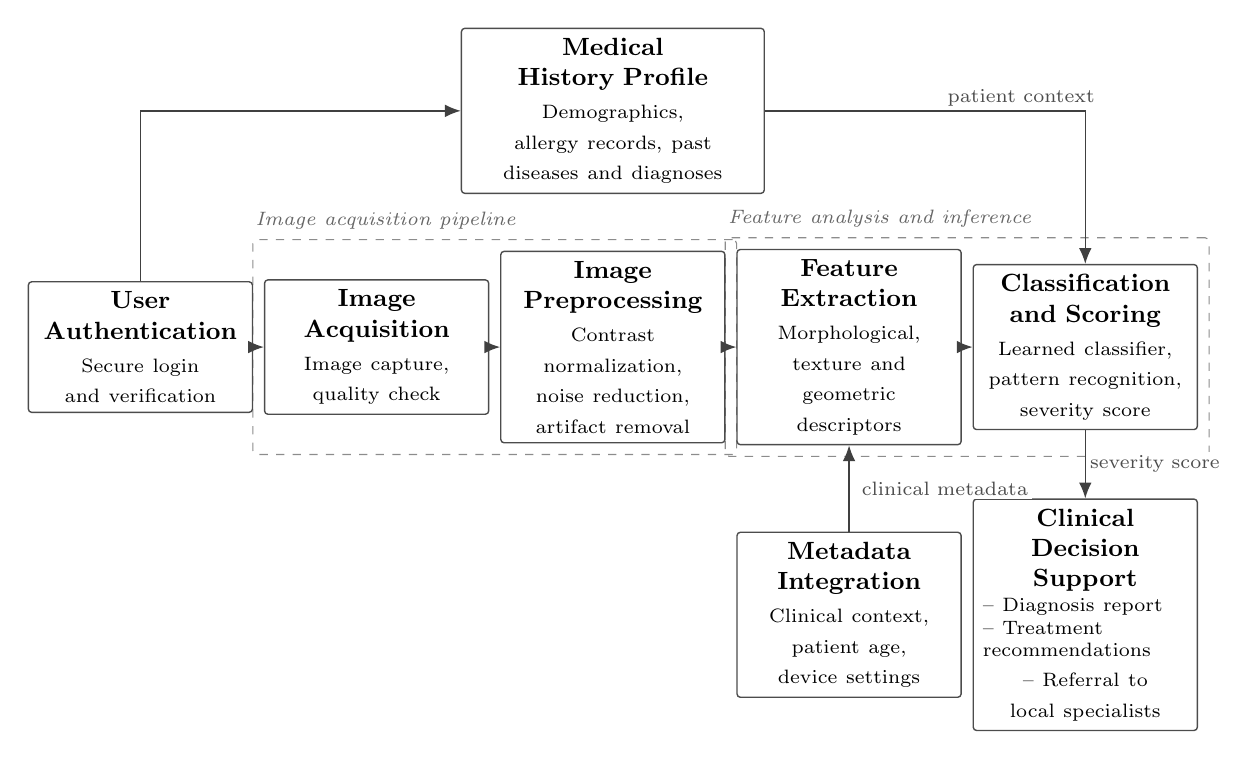
\begin{tikzpicture}[
  font=\small,
  modbox/.style={
    draw=black!70, line width=0.5pt, rounded corners=1.2pt,
    align=center, inner sep=3.5pt,
    text width=26mm, minimum height=14mm},
  grouplabel/.style={font=\scriptsize\itshape, text=black!60, fill=white, inner sep=1pt},
  flow/.style={-{Latex[length=2mm,width=1.6mm]}, draw=black!75, line width=0.5pt},
  edgelab/.style={font=\scriptsize, text=black!70, fill=white, inner sep=1.5pt}
]

% suppress hyphenation inside diagram boxes
\hyphenpenalty=10000\exhyphenpenalty=10000\relax

% ---- main horizontal chain -------------------------------------------
\node[modbox] at (-60mm,0) (auth) {%
  {\small\bfseries User Authentication}\\[1pt]
  {\scriptsize Secure login and verification}};

\node[modbox] at (-30mm,0) (acq) {%
  {\small\bfseries Image Acquisition}\\[1pt]
  {\scriptsize Image capture, quality check}};

\node[modbox] at (0mm,0) (pre) {%
  {\small\bfseries Image Preprocessing}\\[1pt]
  {\scriptsize Contrast normalization, noise reduction, artifact removal}};

\node[modbox] at (30mm,0) (feat) {%
  {\small\bfseries Feature Extraction}\\[1pt]
  {\scriptsize Morphological, texture and geometric descriptors}};

\node[modbox] at (60mm,0) (clf) {%
  {\small\bfseries Classification and Scoring}\\[1pt]
  {\scriptsize Learned classifier, pattern recognition, severity score}};

% ---- medical history profile (above) ---------------------------------
\node[modbox, text width=36mm] at (0mm,30mm) (hist) {%
  {\small\bfseries Medical History Profile}\\[1pt]
  {\scriptsize Demographics, allergy records, past diseases and diagnoses}};

% ---- metadata and clinical decision support (below) ------------------
\node[modbox] at (30mm,-34mm) (meta) {%
  {\small\bfseries Metadata Integration}\\[1pt]
  {\scriptsize Clinical context, patient age, device settings}};

\node[modbox, minimum height=18mm] at (60mm,-34mm) (cds) {%
  {\small\bfseries Clinical Decision Support}\\[1pt]
  {\scriptsize \raggedright
   -- Diagnosis report\\
   -- Treatment recommendations\\
   -- Referral to local specialists}};

% ---- dashed group boxes ----------------------------------------------
\begin{scope}[on background layer]
  \node[draw=black!45, dashed, line width=0.4pt, rounded corners=1.5pt,
        fit=(acq)(pre), inner sep=4pt] (grpA) {};
  \node[draw=black!45, dashed, line width=0.4pt, rounded corners=1.5pt,
        fit=(feat)(clf), inner sep=4pt] (grpB) {};
\end{scope}
\node[grouplabel, anchor=south west] at ([yshift=0.8mm]grpA.north west)
  {Image acquisition pipeline};
\node[grouplabel, anchor=south west] at ([yshift=0.8mm]grpB.north west)
  {Feature analysis and inference};

% ---- connections ------------------------------------------------------
\draw[flow] (auth) -- (acq);
\draw[flow] (acq)  -- (pre);
\draw[flow] (pre)  -- (feat);
\draw[flow] (feat) -- (clf);

% authentication opens the medical history profile
\draw[flow] (auth.north) |- (hist.west);

% history profile supplies patient context to the classifier
\draw[flow] (hist.east) -| (clf.north)
  node[edgelab, pos=0.4, above] {patient context};

% metadata integration feeds feature analysis
\draw[flow] (meta.north) -- (feat.south)
  node[edgelab, midway, right, xshift=1mm] {clinical metadata};

% classification feeds clinical decision support
\draw[flow] (clf.south) -- (cds.north)
  node[edgelab, midway, right] {severity score};

\end{tikzpicture}%
}
\caption{Overview of the complete Intelligent Preliminary Diagnosis (IPD) system pipeline.}
\label{fig:pipeline}
\end{figure}

\subsection{Image Acquisition}

The image acquisition module receives clinical photographs acquired with a smartphone or
general-purpose camera, as well as dermoscopic images acquired with standard dermatoscopy
hardware where such equipment is available \cite{ref23} and performs an automated Image
Quality Check before downstream processing. This check evaluates the acquired images against
heuristic thresholds for resolution, focus sharpness, illumination uniformity and
field-of-view completeness.

\subsection{Image Preprocessing}

Validated images are sent to the preprocessing module and pass through a three-stage
normalisation pipeline. First, contrast normalisation is performed using Contrast Limited
Adaptive Histogram Equalization (CLAHE). Second, noise reduction is achieved through
Gaussian smoothing and median filtering. Third, artifact removal eliminates structured
non-dermatological elements such as ruler markings, ink annotations and lens vignetting.

\subsection{Feature Extraction}

Quality-checked and preprocessed images are passed to the feature extraction stage, which is
realised by the multi-branch deep encoder described in Section~\ref{sec:dlarch}. Rather than
computing handcrafted morphological, texture and geometric descriptors, the system learns its
representations directly from pixels: three heterogeneous encoders operate on the same input
in parallel and produce complementary embeddings that are subsequently projected into a
shared space and fused. The design rationale for this choice, together with the individual
branches, is set out in Section~\ref{sec:encoder}.

\subsection{Metadata Integration}

In parallel with feature extraction from the images, the Metadata Integration module
assembles a structured clinical context vector from three information streams: clinical
context, patient age and device settings \cite{ref7}. Within the deployed IPD system these
metadata features are appended to the visual feature vector before the classification head.
It should be noted that the experiments reported in Section~\ref{sec:results} evaluate the
image-only classification engine of Fig.~\ref{fig:architecture}, since the aggregated public
corpora used in this study do not carry a consistent metadata schema across all five sources;
metadata fusion is therefore specified as part of the system architecture but is not
exercised in the present evaluation.

\subsection{Classification and Scoring}

The fused feature representation is sent to the classification module, which performs
classification using the proposed ensemble deep learning architecture described in
Section~\ref{sec:dlarch}. The module produces (i) a class probability distribution across the
five target conditions, (ii) a Pattern Recognition score that quantifies structural
similarity and (iii) a Severity Assessment index.

\subsection{Clinical Decision Support}

The terminal module converts the classification results into actionable clinical outputs. The
Diagnosis Report lists the top-K conditions ranked by posterior probability. Treatment
Recommendations are derived from an evidence-based knowledge base. Relevant Local Specialists
and Services are identified using a geo-indexed directory, addressing the critical last-mile
referral gap.

\section{Dataset Description}\label{sec:dataset}

One of the major challenges in developing skin disease detection systems for the Indian
population is the lack of representative datasets. The majority of publicly available
dermatological datasets are biased towards lighter Fitzpatrick skin types (Type I--II), while
wheatish to brown skin tones (Type III--V) are under-represented to a large extent. The
constituent sources differ in acquisition modality: Fitzpatrick17k, PAD-UFES-20, DermaCon-IN
and the Skin Disease Image Dataset consist predominantly of clinical photographs, including
smartphone-acquired images, whereas the Melanoma Cancer Image Dataset contributes dermoscopic
imagery. In response, a curated dataset was created from five of the main publicly available
image sets: the Fitzpatrick17k dataset, the PAD-UFES-20 dataset, the DermaCon-IN dataset
\cite{ref5}, the Melanoma Cancer Image Dataset and the Skin Disease Image Dataset (SDID).

\subsection{Data Curation Pipeline}

The dataset was created using a multi-stage preprocessing and filtering procedure that
ensured both quality and skin tone relevance. Skin tone filtering was performed using a
hybrid method: metadata-based filtering was applied to datasets that carry Fitzpatrick skin
type annotations, while image-based filtering in the HSV colour space was applied to datasets
without such annotations. Quality controls included the exclusion of watermarks,
multi-subject images and AI-generated content.

\subsection{Final Dataset Composition}

After applying the pipeline, a final curated dataset of 14,498 images was obtained, divided
into five clinically relevant disease classes as shown in Table~\ref{tab:dataset}.

\begin{table}[htbp]
\caption{Class-wise distribution of the final curated dataset.}\label{tab:dataset}
\begin{tabular}{@{}lr@{}}
\toprule
Disease Class & Number of Images \\
\midrule
Basal Cell Carcinoma & 3372 \\
Eczema & 1788 \\
Keratosis & 2380 \\
Melanoma & 5808 \\
Tinea & 1150 \\
\midrule
Total & 14,498 \\
\botrule
\end{tabular}
\end{table}

\subsection{Data Partitioning and Class Imbalance}\label{sec:imbalance}

The curated corpus was divided into training, validation and test partitions in the ratio
70:15:15, using a fixed random seed of 32 so that the split is reproducible. Partitioning was
stratified by disease class so that the class proportions of Table~\ref{tab:dataset} are
preserved in every partition.

The corpus is imbalanced: Melanoma contributes 5,808 images while Tinea contributes 1,150, a
ratio of approximately five to one. Three complementary mechanisms are used to prevent this
skew from being absorbed into the trained model.

First, mini-batches are constructed using a weighted random sampler rather than uniform
shuffling. Each training instance belonging to class $k$ is assigned a sampling weight
inversely proportional to the frequency of that class
\begin{equation}
w^{\mathrm{samp}}_{k} = \frac{1}{n_{k}}
\end{equation}
where $n_{k}$ is the number of training images of class $k$, and instances are drawn with
replacement. Every mini-batch therefore contains an approximately uniform mixture of the five
conditions irrespective of their prevalence in the corpus. This mechanism governs exposure:
it guarantees that the minority classes appear often enough for their gradients to accumulate.

Second, the classification loss is itself class-weighted. Base weights follow an inverse
square-root frequency rule
\begin{equation}
w_{k} \propto \frac{1}{\sqrt{n_{k}}}
\end{equation}
which is a gentler correction than inverse frequency and avoids over-amplifying the smallest
class once the sampler has already equalised exposure. The normalised weights are then scaled
by condition-specific factors that reflect clinical priority rather than prevalence, after
which the vector is renormalised to sum to unity.

The asymmetry of these factors is deliberate. Melanoma is boosted despite being the majority
class, because the cost of a missed melanoma is not symmetric with the cost of an unnecessary
referral; since the sampler has already equalised how often each class is seen, the loss
weight expresses how much each error matters rather than how often it occurs. Tinea receives
the largest boost as the smallest class and the one most prone to underfitting. The two
mechanisms thus operate on different axes: the sampler ensures that rare classes are
physically present in training, while the weighted loss ensures that the optimiser remains
disproportionately sensitive to errors on the clinically critical conditions.

Third, model selection is itself made imbalance-aware, as described in
Section~\ref{sec:expsetup}. Per-class metrics are reported in addition to overall accuracy so
that performance on the minority classes remains visible.

\section{Deep Learning Architecture}\label{sec:dlarch}

The core classification engine of the IPD system is a heterogeneous multi-branch ensemble
architecture that takes advantage of the complementary inductive biases of convolutional,
attention-based and hybrid families of neural networks. The proposed model accepts clinical
and dermoscopic images resized to a standard spatial resolution of $224 \times 224 \times 3$
pixels.

\subsection{Multi-Branch Encoder Design}\label{sec:encoder}

Let $X \in \mathbb{R}^{224 \times 224 \times 3}$ denote the pre-processed input image. The
input tensor is processed simultaneously by three separate encoder branches:

\begin{itemize}
\item \textbf{EfficientNet-B1 (Primary Edge Detection Module):} uses Mobile Inverted
Bottleneck Convolution (MBConv) blocks with depthwise separable convolutions to extract
fine-grained spatial detail, augmented by a Squeeze-and-Excitation (SE) sub-module
\cite{ref27}.
\item \textbf{Swin Transformer (Primary Pattern Recognition Module):} captures long-range
spatial dependencies through a Shifted Window Multi-head Self-Attention (SW-MSA) mechanism
\cite{ref11}.
\item \textbf{ConvNeXt-Tiny (Secondary Refinement Branch):} uses large-kernel ($7 \times 7$)
depthwise convolutions and Layer Normalization to link local CNN representations with global
transformer representations \cite{ref12}.
\end{itemize}

\begin{figure}[!t]
\centering
% ---------------------------------------------------------------------
% Fig. 2 -- Multi-branch Ensemble Deep Learning Architecture
% Wrapped in \resizebox so the tall/wide TikZ diagram fits the Springer
% text block.
% ---------------------------------------------------------------------
\resizebox{\textwidth}{!}{%
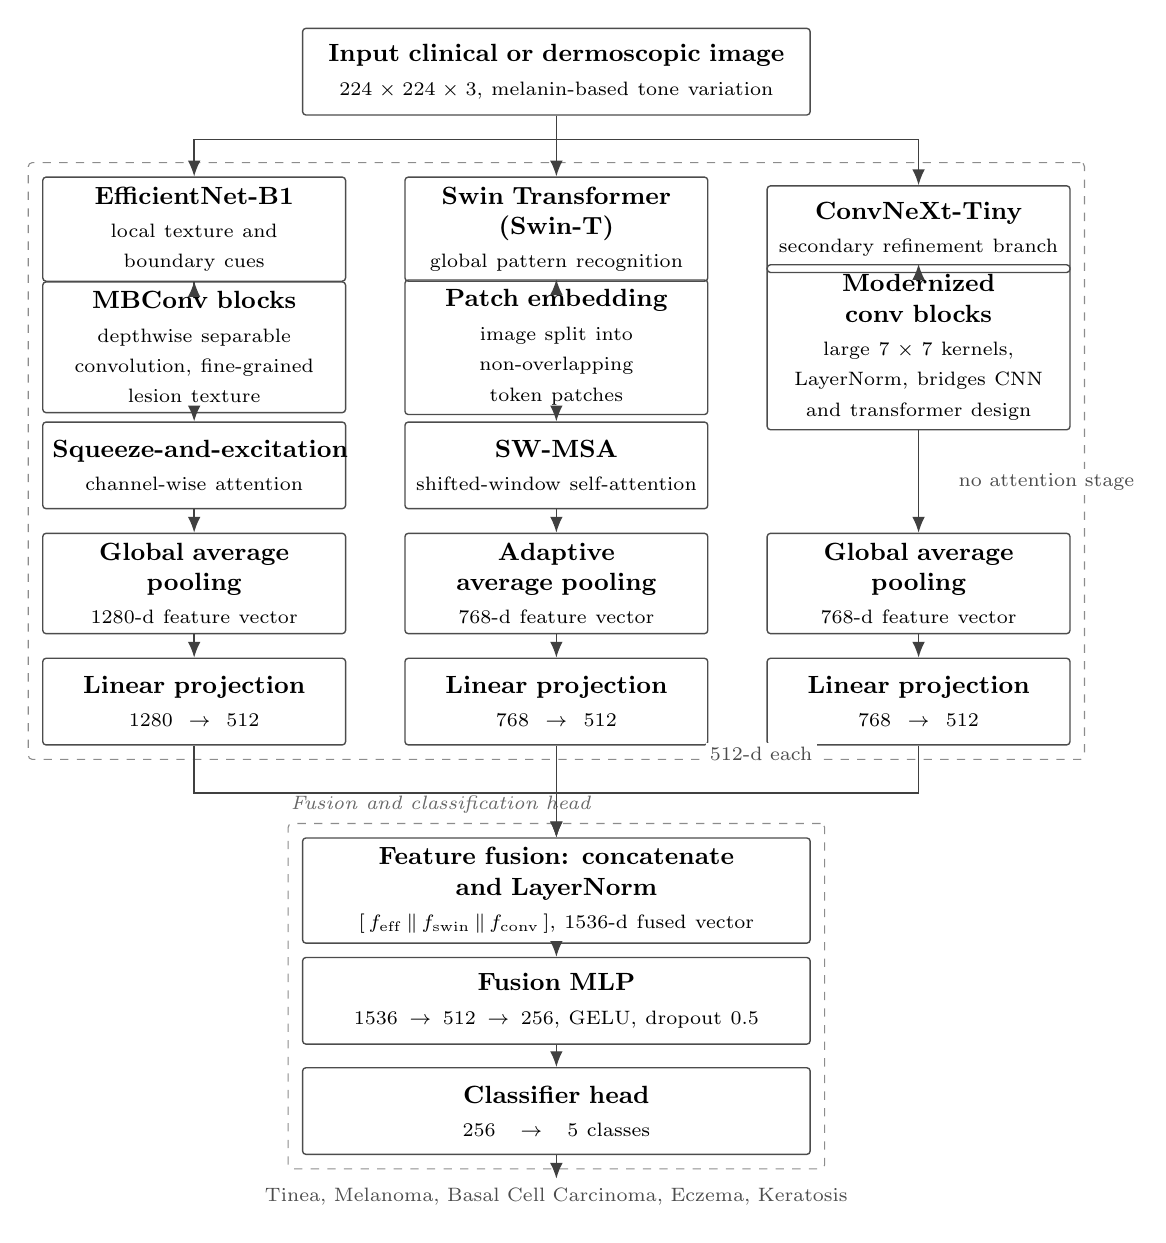
\begin{tikzpicture}[
  font=\small,
  blk/.style={
    draw=black!70, line width=0.5pt, rounded corners=1.2pt,
    align=center, inner sep=3.5pt,
    text width=36mm, minimum height=11mm},
  wide/.style={blk, text width=62mm},
  grouplabel/.style={font=\scriptsize\itshape, text=black!60, fill=white, inner sep=1pt},
  flow/.style={-{Latex[length=2mm,width=1.6mm]}, draw=black!75, line width=0.5pt},
  edgelab/.style={font=\scriptsize, text=black!70, fill=white, inner sep=1.5pt},
  ylev/.style={},
]

% suppress hyphenation inside diagram boxes
\hyphenpenalty=10000\exhyphenpenalty=10000\relax

\def\colA{-46mm}
\def\colB{0mm}
\def\colC{46mm}

% ---- input ----------------------------------------------------------
\node[wide] at (\colB,0) (input) {%
  {\small\bfseries Input clinical or dermoscopic image}\\[1pt]
  {\scriptsize $224 \times 224 \times 3$, melanin-based tone variation}};

% ---- branch headers -------------------------------------------------
\node[blk] at (\colA,-20mm) (effA) {%
  {\small\bfseries EfficientNet-B1}\\[1pt]
  {\scriptsize local texture and boundary cues}};
\node[blk] at (\colB,-20mm) (swiA) {%
  {\small\bfseries Swin Transformer (Swin-T)}\\[1pt]
  {\scriptsize global pattern recognition}};
\node[blk] at (\colC,-20mm) (conA) {%
  {\small\bfseries ConvNeXt-Tiny}\\[1pt]
  {\scriptsize secondary refinement branch}};

% ---- stage 2 --------------------------------------------------------
\node[blk] at (\colA,-35mm) (effB) {%
  {\small\bfseries MBConv blocks}\\[1pt]
  {\scriptsize depthwise separable convolution, fine-grained lesion texture}};
\node[blk] at (\colB,-35mm) (swiB) {%
  {\small\bfseries Patch embedding}\\[1pt]
  {\scriptsize image split into non-overlapping token patches}};
\node[blk] at (\colC,-35mm) (conB) {%
  {\small\bfseries Modernized conv blocks}\\[1pt]
  {\scriptsize large $7 \times 7$ kernels, LayerNorm, bridges CNN and transformer design}};

% ---- stage 3 --------------------------------------------------------
\node[blk] at (\colA,-50mm) (effC) {%
  {\small\bfseries Squeeze-and-excitation}\\[1pt]
  {\scriptsize channel-wise attention}};
\node[blk] at (\colB,-50mm) (swiC) {%
  {\small\bfseries SW-MSA}\\[1pt]
  {\scriptsize shifted-window self-attention}};

% ---- stage 4: pooling ----------------------------------------------
\node[blk] at (\colA,-65mm) (effD) {%
  {\small\bfseries Global average pooling}\\[1pt]
  {\scriptsize 1280-d feature vector}};
\node[blk] at (\colB,-65mm) (swiD) {%
  {\small\bfseries Adaptive average pooling}\\[1pt]
  {\scriptsize 768-d feature vector}};
\node[blk] at (\colC,-65mm) (conD) {%
  {\small\bfseries Global average pooling}\\[1pt]
  {\scriptsize 768-d feature vector}};

% ---- stage 5: projections ------------------------------------------
\node[blk] at (\colA,-80mm) (effE) {%
  {\small\bfseries Linear projection}\\[1pt]
  {\scriptsize $1280 \rightarrow 512$}};
\node[blk] at (\colB,-80mm) (swiE) {%
  {\small\bfseries Linear projection}\\[1pt]
  {\scriptsize $768 \rightarrow 512$}};
\node[blk] at (\colC,-80mm) (conE) {%
  {\small\bfseries Linear projection}\\[1pt]
  {\scriptsize $768 \rightarrow 512$}};

% ---- fusion head ----------------------------------------------------
\node[wide] at (\colB,-104mm) (fuse) {%
  {\small\bfseries Feature fusion: concatenate and LayerNorm}\\[1pt]
  {\scriptsize $[\,f_{\mathrm{eff}} \,\|\, f_{\mathrm{swin}} \,\|\, f_{\mathrm{conv}}\,]$, 1536-d fused vector}};

\node[wide] at (\colB,-118mm) (mlp) {%
  {\small\bfseries Fusion MLP}\\[1pt]
  {\scriptsize $1536 \rightarrow 512 \rightarrow 256$, GELU, dropout 0.5}};

\node[wide] at (\colB,-132mm) (head) {%
  {\small\bfseries Classifier head}\\[1pt]
  {\scriptsize $256 \rightarrow 5$ classes}};

\node[font=\scriptsize, text=black!70, below=3mm of head] (classes)
  {Tinea, Melanoma, Basal Cell Carcinoma, Eczema, Keratosis};

% ---- dashed group boxes ---------------------------------------------
\begin{scope}[on background layer]
  \node[draw=black!45, dashed, line width=0.4pt, rounded corners=1.5pt,
        fit=(effA)(conA)(effE)(conE), inner sep=5pt] (grpBranch) {};
  \node[draw=black!45, dashed, line width=0.4pt, rounded corners=1.5pt,
        fit=(fuse)(head), inner sep=5pt] (grpHead) {};
\end{scope}
\node[grouplabel, anchor=south west] at ([yshift=0.8mm]grpHead.north west) {Fusion and classification head};

% ---- connections -----------------------------------------------------
\draw[flow] (input.south) -- ++(0,-3mm) -| (effA.north);
\draw[flow] (input.south) -- (swiA.north);
\draw[flow] (input.south) -- ++(0,-3mm) -| (conA.north);

\foreach \a/\b in {effA/effB, effB/effC, effC/effD, effD/effE,
                   swiA/swiB, swiB/swiC, swiC/swiD, swiD/swiE,
                   conB/conD, conD/conE}
  \draw[flow] (\a) -- (\b);

\draw[flow] (conA) -- (conB);
\node[edgelab, right=0.5mm] at ($(conB.south)!0.5!(conD.north)+(4mm,0)$) {no attention stage};

\draw[flow] (effE.south) |- ++(0,-6mm) -| (fuse.north);
\draw[flow] (swiE.south) -- (fuse.north);
\draw[flow] (conE.south) |- ++(0,-6mm) -| (fuse.north);
\node[edgelab] at ($(swiE.south)+(26mm,-1mm)$) {512-d each};

\draw[flow] (fuse) -- (mlp);
\draw[flow] (mlp)  -- (head);
\draw[flow] (head) -- (classes);

\end{tikzpicture}%
}
\caption{Multi-branch Ensemble Deep Learning Architecture.}
\label{fig:architecture}
\end{figure}

The MBConv blocks of the first branch factorise a standard convolution into a depthwise and a
pointwise stage. For an input feature map $U$ with $C$ channels, the depthwise stage applies a
single kernel per channel
\begin{equation}
Y_{i,j,c} = \sum_{m} \sum_{n} K^{d}_{m,n,c}\, U_{i+m,\, j+n,\, c},
\qquad c = 1, \ldots, C
\end{equation}
after which a pointwise kernel $K^{p}$ mixes information across channels, $Z = K^{p} * Y$.
This factorisation reduces the parameter count by roughly a factor of $C$ relative to a dense
convolution of the same receptive field, which is what allows the branch to remain narrow
while operating at high spatial resolution.

Channel recalibration is then performed by the Squeeze-and-Excitation sub-module. The squeeze
operation summarises each channel by global average pooling
\begin{equation}
z_{c} = \frac{1}{H \times W} \sum_{i=1}^{H} \sum_{j=1}^{W} u_{c}(i,j)
\end{equation}
and the excitation operation learns a multiplicative gate over channels
\begin{equation}
s = \sigma\!\left(W_{2}\, \delta(W_{1} z)\right), \qquad \tilde{u}_{c} = s_{c}\, u_{c}
\end{equation}
where $\delta$ denotes the ReLU non-linearity, $\sigma$ the logistic sigmoid, and
$W_{1} \in \mathbb{R}^{\frac{C}{r} \times C}$,
$W_{2} \in \mathbb{R}^{C \times \frac{C}{r}}$ with reduction ratio $r$. In melanin-rich
imagery, where lesion boundaries are frequently expressed through texture rather than colour
contrast, this gating allows the branch to suppress channels dominated by background
pigmentation.

The second branch partitions the feature map into non-overlapping windows and computes
self-attention within each window
\begin{equation}
\mathrm{Attention}(Q,K,V) = \mathrm{softmax}\!\left(\frac{QK^{\top}}{\sqrt{d}} + B\right) V
\end{equation}
where $Q$, $K$ and $V$ are the query, key and value projections of the window tokens, $d$ is
the query dimension and $B$ is the learned relative position bias. Consecutive Swin blocks
alternate between regular and shifted window partitioning so that information crosses window
boundaries
\begin{align}
\hat{z}^{\,l} &= \mathrm{W\text{-}MSA}\!\left(\mathrm{LN}\!\left(z^{l-1}\right)\right) + z^{l-1} \\
z^{l} &= \mathrm{MLP}\!\left(\mathrm{LN}\!\left(\hat{z}^{\,l}\right)\right) + \hat{z}^{\,l} \\
\hat{z}^{\,l+1} &= \mathrm{SW\text{-}MSA}\!\left(\mathrm{LN}\!\left(z^{l}\right)\right) + z^{l} \\
z^{l+1} &= \mathrm{MLP}\!\left(\mathrm{LN}\!\left(\hat{z}^{\,l+1}\right)\right) + \hat{z}^{\,l+1}
\end{align}

The third branch applies an inverted-bottleneck residual block in which a large-kernel
depthwise convolution is followed by Layer Normalization and two pointwise projections
separated by a GELU non-linearity
\begin{equation}
y = x + W_{p2}\, \mathrm{GELU}\!\left(W_{p1}\, \mathrm{LN}\!\left(\mathrm{DWConv}_{7\times7}(x)\right)\right)
\end{equation}

Each branch terminates in a pooling operation that reduces its final feature map to a vector
\begin{equation}
f_{b} = \frac{1}{H_{b} \times W_{b}} \sum_{i=1}^{H_{b}} \sum_{j=1}^{W_{b}} X_{b}(i,j,\cdot),
\qquad b \in \{\mathrm{eff}, \mathrm{swin}, \mathrm{conv}\}
\end{equation}
yielding $f_{\mathrm{eff}} \in \mathbb{R}^{1280}$, $f_{\mathrm{swin}} \in \mathbb{R}^{768}$
and $f_{\mathrm{conv}} \in \mathbb{R}^{768}$.

\subsection{Feature Fusion via Concatenation and LayerNorm}

Because the three branches emit vectors of differing dimensionality and scale, each is mapped
into a common 512-dimensional space by a learned linear projection
\begin{equation}
\tilde{f}_{b} = W_{b} f_{b} + c_{b}, \qquad W_{b} \in \mathbb{R}^{512 \times d_{b}},
\qquad d_{b} \in \{1280, 768, 768\}
\end{equation}
The three projected embeddings are concatenated and normalised to produce the fused
representation
\begin{equation}
f_{\mathrm{fused}} = \mathrm{LN}\!\left[\tilde{f}_{\mathrm{eff}} \,\|\, \tilde{f}_{\mathrm{swin}}
\,\|\, \tilde{f}_{\mathrm{conv}}\right] \in \mathbb{R}^{1536}
\end{equation}
where $\|$ denotes concatenation along the feature axis. Layer Normalization is applied after
concatenation rather than before it, so that the three sub-vectors are placed on a common
scale and no branch dominates the fused representation purely by virtue of larger activation
magnitudes \cite{ref13}.

\subsection{Fusion MLP and Classification Head}

The fused vector is compressed by a two-layer Fusion Multilayer Perceptron with GELU
activations and dropout
\begin{equation}
h_{1} = \mathrm{GELU}(W_{1} f_{\mathrm{fused}} + b_{1}), \qquad
h_{2} = \mathrm{Dropout}_{0.5}\!\left(\mathrm{GELU}(W_{2} h_{1} + b_{2})\right)
\end{equation}
with $W_{1} \in \mathbb{R}^{512 \times 1536}$ and $W_{2} \in \mathbb{R}^{256 \times 512}$, so
that the representation is reduced from 1536 to 256 units. A fully connected classifier head
then produces the logit vector $z = W_{c} h_{2} + b_{c}$ over the $K = 5$ target classes, and
the predicted class distribution follows from the softmax
\begin{equation}
p_{k} = \frac{\exp(z_{k})}{\sum_{j=1}^{K} \exp(z_{j})}, \qquad k = 1, \ldots, K
\end{equation}

\subsection{Training Configuration and Optimization}\label{sec:training}

The network is trained end-to-end by minimising the cross-entropy loss with label smoothing.
Writing $y$ for the one-hot target, the smoothed target and the resulting objective are
\begin{equation}
q_{k} = (1 - \varepsilon)\, y_{k} + \frac{\varepsilon}{K}, \qquad
\mathcal{L} = -\sum_{k=1}^{K} w_{k}\, q_{k} \log p_{k}
\end{equation}
with $\varepsilon = 0.1$ and $w_{k}$ the class weights defined in
Section~\ref{sec:imbalance}. Smoothing is retained here because several of the target
conditions overlap visually in pigmented skin, and penalising over-confident predictions
discourages the network from committing to a single class on evidence that does not warrant
it.

Parameters are updated with the AdamW optimizer \cite{ref26}, in which weight decay is
decoupled from the gradient-based update
\begin{equation}
\theta_{t} = \theta_{t-1} - \eta \left( \frac{\hat{m}_{t}}{\sqrt{\hat{v}_{t}} + \delta}
+ \lambda\, \theta_{t-1} \right)
\end{equation}
where $\hat{m}_{t}$ and $\hat{v}_{t}$ are the bias-corrected first- and second-moment
estimates of the gradient, $\eta = 3 \times 10^{-4}$ is the initial learning rate,
$\lambda = 1 \times 10^{-4}$ is the weight decay coefficient and $\delta$ is a small constant
for numerical stability. Robust data augmentation is applied throughout training.

\section{Results and Discussion}\label{sec:results}

\subsection{Experimental Setup}\label{sec:expsetup}

All experiments were carried out on a dual NVIDIA T4 configuration provided by the Kaggle
free-tier environment, comprising two T4 accelerators with 16 GB of VRAM each for a combined
32 GB, using PyTorch with CUDA acceleration. Each branch was initialised from
ImageNet-pretrained weights and the network was then fine-tuned for 30 epochs using the AdamW
configuration of Section~\ref{sec:training} and a fixed random seed of 32. Batch sizes were
set per encoder according to memory footprint: 16 for EfficientNet-B1, 12 for ConvNeXt and 8
for the Swin Transformer. Total training time was approximately six hours.

Input images were first resized to $256 \times 256$, that is the 224 target resolution with 32
pixels of padding, from which a random $224 \times 224$ crop was taken so that the network
never observes an identical framing twice. The remaining augmentation pipeline comprised
random horizontal and vertical flips; random rotation of up to $\pm 30^{\circ}$; colour jitter
with brightness 0.4, contrast 0.4, saturation 0.3 and hue 0.1; a random affine transform with
translation up to 10\%, shear of $10^{\circ}$ and scaling between 0.85 and 1.15; and random
greyscale conversion with probability 0.05. Colour jitter and greyscale conversion were
included to encourage invariance to illumination and capture-device variation, which is a
practical concern for a system intended to accept smartphone photographs. Images were then
converted to tensors and normalised using the ImageNet channel statistics, with means of
0.485, 0.456 and 0.406 and standard deviations of 0.229, 0.224 and 0.225. Finally,
cutout-style random erasing was applied after normalisation with probability 0.25, removing a
region covering between 2\% and 20\% of the image at an aspect ratio between 0.3 and 3.3,
which discourages the network from relying on any single localised region of the lesion.

Model selection was deliberately not performed on validation accuracy, since a model favouring
the majority classes can inflate that quantity while performing poorly on the conditions that
matter most. Checkpoints were instead retained according to a composite criterion combining
malignant-class sensitivity with overall accuracy
\begin{equation}
S = 0.4 \cdot \mathrm{Sens}_{\mathrm{mel}} + 0.3 \cdot \mathrm{Sens}_{\mathrm{bcc}}
+ 0.3 \cdot \mathrm{Acc}_{\mathrm{val}}
\end{equation}
so that where two epochs achieve comparable overall accuracy, the one with better melanoma and
basal cell carcinoma recall is the one preserved. This directly counteracts the risk of an
inflated headline accuracy driven by the majority class. Performance is reported in terms of
accuracy, macro-averaged AUC, the Matthews correlation coefficient (MCC), and per-class
precision, recall and F1-score.

\subsection{Comparison with Individual Backbones}\label{sec:comparison}

The proposed ensemble architecture was evaluated against its constituent backbones trained
individually, namely EfficientNet-B1, ConvNeXt-Tiny and Swin-Tiny. The comparison is
summarised in Fig.~\ref{fig:comparison} and the corresponding receiver operating
characteristic curves in Fig.~\ref{fig:roc}.

\begin{figure}[!htbp]
\centering
\includegraphics[width=\textwidth]{fig3_model_comparison.pdf}
\caption{Model Comparison: Test Accuracy, Macro-Average AUC, and MCC.}
\label{fig:comparison}
\end{figure}

The ensemble attains a test accuracy of 85.39\% and a macro-averaged AUC of 0.9762. Relative
to the weaker convolutional baselines the improvement is substantial: ConvNeXt-Tiny reaches
only 71.35\% accuracy with an MCC of 0.6507, and EfficientNet-B1 reaches 84.97\% with an MCC
of 0.8119. Relative to the strongest single backbone the picture is more nuanced and is worth
stating precisely. Swin-Tiny also reaches 85.39\% accuracy, so the ensemble does not improve
on it in accuracy terms; the gains appear instead in the ranking-based and correlation-based
measures, where the ensemble improves macro-AUC from 0.9683 to 0.9762 and MCC from 0.8174 to
0.8178. The margin in MCC in particular is narrow, and is reported here as an observation
rather than as a claim of improvement.

Two observations follow. First, the value of the ensemble in this setting lies less in raising
peak accuracy than in improving the calibration and ranking quality of the predicted class
probabilities, which is what the macro-AUC gain reflects and which matters for a system
intended to present ranked differential diagnoses rather than a single label. Second, the
fused model recovers almost all of the performance of its strongest member while remaining far
less dependent on that member, so that the failure modes of any one architecture are diluted
rather than inherited.

\begin{figure}[!htbp]
\centering
\includegraphics[width=\textwidth]{fig4_roc.jpg}
\caption{ROC Curves for individual classes and macro-averages.}
\label{fig:roc}
\end{figure}

\subsection{Per-Class Performance and Confusion Analysis}\label{sec:perclass}

The confusion matrices of Fig.~\ref{fig:confusion} show that discriminative performance is not
uniform across the five conditions. Basal Cell Carcinoma and Melanoma are classified most
reliably, at per-class sensitivities of 0.97 and 0.96 respectively, which is the clinically
desirable ordering: these are the two malignant categories in the taxonomy, and a missed
malignancy carries a far higher cost than a false referral.

The principal source of residual error is the confusion between Eczema and Tinea, which is
bidirectional: 22\% of Eczema cases are predicted as Tinea and 19\% of Tinea cases are
predicted as Eczema. This is consistent with clinical experience rather than at odds with it.
Both conditions present as scaly, erythematous or hyperpigmented plaques, and in melanin-rich
skin the erythema that would ordinarily distinguish an eczematous plaque is frequently masked,
leaving annular scaling as the main visual cue. In routine practice the two are separated by
potassium hydroxide microscopy rather than by inspection alone, so a purely image-based
classifier is being asked to make a distinction that dermatologists themselves do not attempt
on morphology alone. Keratosis shows the next highest error rate, with 10\% of cases predicted
as Basal Cell Carcinoma, which again mirrors a known clinical overlap between pigmented actinic
keratoses and superficial basal cell carcinomas.

\begin{figure}[!htbp]
\centering
\includegraphics[width=\textwidth]{fig5_confusion_matrix.pdf}
\caption{Confusion Matrix, Agreement Analysis, and Per-Class Sensitivity.}
\label{fig:confusion}
\end{figure}

\subsection{Ablation of Ensemble Branches}\label{sec:ablation}

To establish what the fusion contributes over its constituent parts, each branch was
additionally trained and evaluated in isolation under the identical protocol of
Section~\ref{sec:expsetup}, and compared against the complete three-branch model. The results
are given in Table~\ref{tab:ablation}.

\begin{table}[htbp]
\caption{Comparison of the individual encoder branches and the fused three-branch ensemble
under an identical training protocol.}\label{tab:ablation}
\begin{tabular}{@{}lccc@{}}
\toprule
Configuration & Accuracy & Macro-AUC & MCC \\
\midrule
EfficientNet-B1 only & 84.97\% & 0.9636 & 0.8119 \\
Swin-Tiny only & 85.39\% & 0.9683 & 0.8174 \\
ConvNeXt-Tiny only & 71.35\% & 0.9418 & 0.6507 \\
\midrule
All three branches (proposed) & 85.39\% & 0.9762 & 0.8178 \\
\botrule
\end{tabular}
\end{table}

The comparison shows that the branches are far from equally capable in isolation:
ConvNeXt-Tiny trails the other two by roughly fourteen accuracy points, while EfficientNet-B1
and Swin-Tiny are closely matched. The fused model nevertheless exceeds every individual
branch on macro-AUC and MCC, and matches the best of them on accuracy. The gain therefore
arises from the complementarity of the errors made by the three encoders rather than from the
strength of any one of them, which is the behaviour a fused representation is intended to
produce: a weaker branch can still contribute discriminative evidence on the subset of cases
where the stronger branches are uncertain.

\section{Conclusion}\label{sec:conclusion}

This study addresses the crucial diagnostic gap for dermatological disorders in the
melanin-rich, brown skin tones that are typical of South Asian populations. By introducing an
innovative heterogeneous ensemble learning framework that combines EfficientNet, Swin
Transformer and ConvNeXt architectures, this research effectively mitigated the dataset
biases that traditionally degrade the performance of AI systems on darker skin tones. The
experimental results show that the proposed multi-branch ensemble matches the accuracy of its
strongest individual backbone while improving macro-averaged AUC, and that it retains high
diagnostic sensitivity on the critical malignant conditions, namely Melanoma and Basal Cell
Carcinoma. Although clinical metadata integration is specified as part of the architecture, it
is not exercised in the present image-only evaluation; its integration with deep learning
feature extraction nonetheless outlines a viable route towards clinical deployment that future
work will assess empirically.

\section{Future Scope}\label{sec:future}

Two directions are identified as the immediate continuations of this work.

\begin{enumerate}
\item \textbf{Dataset expansion and clinical deployment.} Future work will emphasise
augmenting the dataset with real-world clinical images from localised demographics and
deploying the clinical decision support system within primary healthcare nodes across India.
\item \textbf{Introducing explainability (XAI) into the ensemble.} In its present form the
proposed model returns a class distribution without indicating which image evidence supports
it, which is a limitation for a system intended to assist rather than replace a clinician. The
next iteration will therefore embed explainability directly within the multi-branch design.
Gradient-weighted class activation mapping can be computed on the convolutional branches and
attention rollout on the shifted window branch, so that each encoder contributes a saliency map
of its own and the maps can be compared against one another as well as aggregated into a single
explanation aligned with the fused prediction \cite{ref21,ref22}. Two benefits are anticipated.
Clinically, a visual justification allows a dermatologist to confirm that the prediction rests
on the lesion itself rather than on background pigmentation, illumination or capture artefacts,
which is precisely the failure mode that melanin-rich imagery makes hard to detect from the
label alone. Diagnostically for the model, disagreement between branch-level saliency maps
offers a route to inspecting the Eczema--Tinea confusion reported in
Section~\ref{sec:perclass}, since it reveals whether the branches are attending to the same
morphological cue when they disagree. Generating the explanation from within the model rather
than imposing it afterwards, in the manner of the inherently explainable formulations
discussed in the literature \cite{ref19,ref20}, is the preferred design, so that the
highlighted region and the predicted class remain spatially consistent.
\end{enumerate}

\begin{thebibliography}{99}

\bibitem{ref1}
Aboulmira, A., Hrimech, H., Lachgar, M.: Skin diseases classification with machine learning
and deep learning techniques: A systematic review. International Journal of Advanced Computer
Science and Applications \textbf{15}(10), 1155--1173 (2024)

\bibitem{ref2}
Yan, S., Yu, Z., Primiero, C., Vico-Alonso, C., Wang, Z., Yang, L., Tschandl, P., Hu, M.,
Ju, L., et al.: A multimodal vision foundation model for clinical dermatology. Nature Medicine
\textbf{31}(8), 2691--2702 (2025)

\bibitem{ref3}
Ward, A., Li, J., Wang, J., Lakshminarasimhan, S., Carrick, A., Campana, B., Hartford, J.,
et al.: Creating an empirical dermatology dataset through crowdsourcing with web search
advertisements. JAMA Network Open \textbf{7}(11), e2446615 (2024)

\bibitem{ref4}
Gottfrois, P., Gr\"{o}ger, F., Andriambololoniaina, F.H., Amruthalingam, L.,
Gonzalez-Jimenez, A., Hsu, C., Kessy, A., Lionetti, S., et al.: PASSION for dermatology:
Bridging the diversity gap with pigmented skin images from Sub-Saharan Africa. In: Medical
Image Computing and Computer Assisted Intervention -- MICCAI 2024, Lecture Notes in Computer
Science, vol. 15003, pp. 703--712. Springer, Cham (2024)

\bibitem{ref5}
Madarkar, S.S., Madarkar, M., Madhumitha, V., Prakash, T., Mopuri, K.R., Vinaykumar, M.V.,
Sathwika, K.V.L., et al.: DermaCon-IN: A multi-concept annotated dermatological image dataset
of Indian skin disorders for clinical AI research. In: Advances in Neural Information
Processing Systems (NeurIPS), Datasets and Benchmarks Track (2025)

\bibitem{ref6}
Ben\v{c}evi\'{c}, M., Habijan, M., Gali\'{c}, I., Babin, D., Pi\v{z}urica, A.: Understanding
skin color bias in deep learning-based skin lesion segmentation. Computer Methods and Programs
in Biomedicine \textbf{245}, 108044 (2024)

\bibitem{ref7}
Corbin, A., Marques, O.: Exploring strategies to generate Fitzpatrick skin type metadata for
dermoscopic images using individual typology angle techniques. Multimedia Tools and
Applications \textbf{82}(15), 23771--23795 (2023)

\bibitem{ref8}
Kong, Q., Chiu, C.-H., Zeng, D., Chen, Y.-J., Ho, T.-Y., Hu, J., Shi, Y.: Achieving fairness
through channel pruning for dermatological disease diagnosis. In: Medical Image Computing and
Computer Assisted Intervention -- MICCAI 2024, pp. 24--34. Springer, Cham (2024)

\bibitem{ref9}
Munia, N., Imran, A.-A.-Z.: DermDiff: Generative diffusion model for mitigating racial biases
in dermatology diagnosis. arXiv preprint arXiv:2503.17536 (2025)

\bibitem{ref10}
Housley, P.P., Samia, A.M., Motaparthi, K.: Performance evaluation of ChatGPT-4o in
dermatological diagnoses across Fitzpatrick skin types. Cureus (2025).
https://doi.org/10.7759/cureus.87368

\bibitem{ref11}
Ayas, S.: Multiclass skin lesion classification in dermoscopic images using Swin Transformer
model. Neural Computing and Applications \textbf{35}(9), 6713--6722 (2023)

\bibitem{ref12}
Hao, S., Zhang, L., Jiang, Y., Wang, J., Ji, Z., Zhao, L., Ganchev, I.: ConvNeXt-ST-AFF: A
novel skin disease classification model based on fusion of ConvNeXt and Swin Transformer.
IEEE Access \textbf{11}, 117460--117473 (2023)

\bibitem{ref13}
Liu, X., Wang, X., Liu, H., Zang, X., Li, L., Ji, Z., Ganchev, I.: FUSCANet: Enhancing skin
disease classification through feature fusion and spatial-channel attention mechanisms. IEEE
Access \textbf{13}, 100683--100698 (2025)

\bibitem{ref14}
Lilhore, U.K., Sharma, Y.K., Simaiya, S., Alroobaea, R., Baqasah, A.M., Alsafyani, M.,
Alhazmi, A.: SkinEHDLF: A hybrid deep learning approach for accurate skin cancer
classification in complex systems. Scientific Reports \textbf{15}, 14913 (2025)

\bibitem{ref15}
Thwin, S.M., Park, H.-S.: Skin lesion classification using a deep ensemble model. Applied
Sciences \textbf{14}(13), 5599 (2024)

\bibitem{ref16}
Thwin, S.M., Park, H.-S.: Enhanced skin lesion segmentation and classification through
ensemble models. Eng \textbf{5}(4), 2805--2820 (2024)

\bibitem{ref17}
Asif, S., Zhao, M., Li, Y., Tang, F., Zhu, Y.: CFI-Net: A Choquet fuzzy integral based
ensemble network with PSO-optimized fuzzy measures for diagnosing multiple skin diseases
including Mpox. IEEE Journal of Biomedical and Health Informatics \textbf{28}(9), 5573--5586
(2024)

\bibitem{ref18}
Gururaj, H.L., Manju, N., Nagarjun, A., Manjunath Aradhya, V.N., Flammini, F.: DeepSkin: A
deep learning approach for skin cancer classification. IEEE Access \textbf{11}, 50205--50214
(2023)

\bibitem{ref19}
Hosny, K.M., Said, W., Elmezain, M., Kassem, M.A.: Explainable deep inherent learning for
multi-classes skin lesion classification. Applied Soft Computing \textbf{159}, 111624 (2024)

\bibitem{ref20}
Metta, C., Beretta, A., Guidotti, R., Yin, Y., Gallinari, P., Rinzivillo, S., Giannotti, F.:
Advancing dermatological diagnostics: Interpretable AI for enhanced skin lesion classification.
Diagnostics \textbf{14}(7), 753 (2024)

\bibitem{ref21}
Badhon, S.M.S.I., Khushbu, S.A., Shaqib, S.M., Ali, M.A., Anik, A.H., Hossain, K.S.M.T.:
Explainable AI for skin disease classification using gradient-weighted class activation mapping
and transfer learning in digital health to identify contours. Digital Health \textbf{11} (2025)

\bibitem{ref22}
Fiaz, M., Khan, M.B.S., Khan, A.H., Bilal, A., Abdullah, M., Darem, A.A., Sarwar, R.: An
explainable hybrid deep learning framework for precise skin lesion segmentation and multi-class
classification. Frontiers in Medicine \textbf{12} (2025)

\bibitem{ref23}
Lee, K., Cavalcanti, T.C., Kim, S., Lew, H.M., Suh, D.H., Lee, D.H., Hwang, J.Y.: Multi-task
and few-shot learning-based fully automatic deep learning platform for mobile diagnosis of skin
diseases. IEEE Journal of Biomedical and Health Informatics \textbf{27}(1), 176--187 (2023)

\bibitem{ref24}
Hossen, Md.N., Panneerselvam, V., Koundal, D., Ahmed, K., Bui, F.M., Ibrahim, S.M.: Federated
machine learning for detection of skin diseases and enhancement of Internet of Medical Things
(IoMT) security. IEEE Journal of Biomedical and Health Informatics \textbf{27}(2), 835--841
(2023)

\bibitem{ref25}
Hsu, B.W.-Y., Tseng, V.S.: HiTrace: Hierarchical class tracing approach for open-set
recognition on skin lesions. IEEE Journal of Biomedical and Health Informatics \textbf{29}(8),
5700--5711 (2025)

\bibitem{ref26}
Loshchilov, I., Hutter, F.: Decoupled weight decay regularization. In: International Conference
on Learning Representations (ICLR) (2019)

\bibitem{ref27}
Hu, J., Shen, L., Sun, G.: Squeeze-and-excitation networks. In: Proceedings of the IEEE
Conference on Computer Vision and Pattern Recognition (CVPR), pp. 7132--7141 (2018)

\end{thebibliography}

\end{document}